\documentclass[dvipdfmx,11pt]{beamer}		% for my notebook computer and my Mac computer
%\documentclass[11pt]{beamer}			% for overleaf

\usepackage{amsmath}
\usepackage{amssymb}
%\usepackage{amsthm}
\usepackage{multicol}
\usepackage{listings}
\usepackage{otf}
\usepackage{enumerate}
\usepackage{algorithm}
\usepackage{algorithmic}
\usepackage{tikz}
\usepackage{mathtools}
\usepackage{comment}
\usetheme{Berlin}	%全体のデザイン

\useoutertheme[subsection=false]{smoothbars}	%デザインのカスタマイズ

\setbeamertemplate{navigation symbols}{}	%右下のちっちゃいナビゲーション記号を非表示

\AtBeginSubsection[]	%サブセクションごとに目次を表示
{\begin{frame}{Contents}
    \begin{multicols}{2}
        \tableofcontents[currentsubsection]
    \end{multicols}
\end{frame}}

\newtheorem{defi}{Definition}
\newtheorem{thm}[defi]{Theorem}
\newtheorem{prop}[defi]{Proposition}
\newtheorem{conj}[defi]{Conjecture}
\newtheorem{exam}[defi]{Example}
\newtheorem{prob}[defi]{Problem}
\newtheorem{set}[defi]{Setting}
\newtheorem{claim}[defi]{Claim}
\newtheorem{cor}[defi]{Corollary}
\newcommand{\N}{\mathbb{N}}
\newcommand{\R}{\mathbb{R}}
\newcommand{\Z}{\mathbb{Z}}
\newcommand{\X}{\mathcal{X}}
\newcommand{\Y}{\mathcal{Y}}
\newcommand{\Hil}{\mathcal{H}}
\newcommand{\Loss}{\mathcal{L}_{\mathbb{D}}}
\newcommand{\MLsp}{(\X, \Y, \mathbb{D}, \Hil, \Loss)}
\newcommand{\GAN}{(\X, \Y, \mathbb{D}, \Hil_{G}\times\Hil_{D}, \Loss)}
\newcommand{\argmax}{\mathop{\rm arg~max}\limits}
\newcommand{\argmin}{\mathop{\rm arg~min}\limits}

%---------------数理最適化--------------
\newcounter{mpproblem}[section]
\renewcommand{\thempproblem}{\thesection.\arabic{mpproblem}}
\makeatletter
\newenvironment{mpproblem}[1]%
{%
    \protected@edef\@currentlabelname{#1}%
    \par\vspace{\baselineskip}\noindent%
    \ifx#1\empty %
    \else \refstepcounter{mpproblem}$($#1$)$ %
    \fi%
    \hfill%
    $\left|%
    \hfill%
    \hspace{0.00\textwidth}%
    \@fleqntrue\@mathmargin\parindent%
    \begin{minipage}{0.86\textwidth}%
    \vspace{-1.0\baselineskip}%
}%
{%
    \end{minipage}%
    \@fleqnfalse%
    \right.$%
    \par\vspace{\baselineskip}\noindent%
    \ignorespacesafterend%
}%
\makeatother
\newcommand{\mpprobref}[1]{$($\nameref{#1}$)$}

\newenvironment{mpproblem*}%
{%
    \begin{mpproblem}{}%
}%
{%
    \end{mpproblem}%
    \ignorespacesafterend%
}
%-----------------------------------

\title{Optimization Algorithms on Riemannian Manifolds and their Applications}
\author{小泉 孝弥}
\institute{立命館大学理工学部数理科学科4回生}
\date{2021年3月15日 (月曜日)\\ 13:30$\sim$14:30}
\begin{document}
    \begin{frame}\frametitle{}
        \titlepage
    \end{frame}
    \section*{Contents}
    \begin{frame}\frametitle{Contents}
        \begin{multicols}{2}
            \tableofcontents
        \end{multicols}
    \end{frame}
\section{About Optimization}
    \subsection{Optimization Problem}
    \begin{frame}
        \frametitle{最適化問題とは}
        \begin{block}{最適化問題}
            $M$を$\R^n$の部分集合とする. 関数$f : \R^n\to\R$を$M$に制限した時に
            最大となる点$x^*\in M$を求める問題を最大化問題, 最小となる点$x_*\in M$
            を求める問題を最小化問題という. 最大化問題・最小化問題を合わせて(連続)最適化問題(Optimization Problem)といい, 
            この時の$f$を目的関数(objective function), $M$を制約空間(Constraint space)と呼ぶ. 
        \end{block}
        特に, $M = \R^n$の時, \textbf{制約なし}最適化問題といい, $M\neq\R^n$の時, \textbf{制約つき}最適化問題
        という. また, $f$を$\R^n$上ではなく有限集合$V\subset\Z$上の関数の時の最適化問題を 
        (離散)最適化問題と呼ぶ. 
    \end{frame}
    \begin{frame}
        \frametitle{最適化問題の具体例}
        \begin{exampleblock}{2次関数の最小化(制約なし)}
            $f : \R\to\R$を$f(x) = x^2 + 25x + 12$とする. 
            この$f$が最小となるような点$x^*\in\R$を求めよ.
        \end{exampleblock}
        \begin{exampleblock}{長方形の面積最大化(制約あり)}
            $f : \R^2\to\R$を$f(x, y) = xy$とする. $L\geq 0$とした時, 
            この$f$が最大となるような点$(x^*, y^*)\in M = \{(x, y)\mid x\geq 0, y\geq0, 2(x + y) = L\}$を求めよ.
        \end{exampleblock}        
    \end{frame}
    \begin{frame}
        \frametitle{最適化数学と現実社会}
        現代社会において, 様々な分野で最適化は必要とされている.
        \begin{exampleblock}{Delivery Scope 問題}
            Covid-19の影響で, 店舗配達の需要が増加し, 店舗の配達可能区域を決める必要性が高まった.
            できるだけ需要を高くした上で, 制限時間の間にお客に商品を届けることができる領域を求める問題.
        \end{exampleblock}
        \begin{exampleblock}{高次元目的関数最適化問題}
            高次元(何千億次元)で複雑な目的関数を最適化する問題(特に, 機械学習). 
        \end{exampleblock} 
    \end{frame}
    \subsection{Optimization Algorithm}
    \begin{frame}
        \frametitle{最適化アルゴリズム}
        最適化問題を解くためにほぼ必須となるのが, \textbf{最適化アルゴリズム} (Optimization Algorithm)である.
        これにより, 最適化問題を計算機に効率的に解かせることができる. 例えば, 目的関数が微分可能で, 制約がない最適化問題であれば
        \textbf{勾配降下法}(Gradient Decent) を使って解くこと(局所的最適解を求める)ができる.
        \begin{algorithm}[H]
            \caption{Gradient Decent(GD)}
            \begin{algorithmic}
                \REQUIRE $f$: differentiable function on $\R^{d}$
                \REQUIRE $0< t <1$ : 
                \STATE $x\leftarrow x_{0}\in\R^n$
                \WHILE{$x$ not converged} 
                \STATE $x\leftarrow x - t~\mathrm{grad} f(x)$ 
                \ENDWHILE
                \RETURN $x$
            \end{algorithmic}
        \end{algorithm}
    \end{frame}
    \begin{frame}
        \frametitle{制約付き最適化問題とリーマン多様体}
        GD法は便利な手法だが, $x\in M$であったとしても, $x - t~\mathrm{grad} f(x)\in M$
        となるとは限らないため, GD法を中心とした制約なし最適化問題用のアルゴリズムを制約付き最適化問題
        に用いることはできない. しかしながら, $M$がリーマン多様体である時は, $f$の定義域を$M$に制限することにより
        制約なしの最適化問題とみなすことで, これらのアルゴリズムをリーマン多様体に拡張したものを適用することができる. 
    \end{frame}
\section{Riemannian Manifolds}
    \subsection{Riemannian Manifold and Gradient}
    \begin{frame}
        \frametitle{Riemannian Manifold}
        \begin{defi}[Riemannian Manifold]
            $M$を可微分多様体とする. 任意の$x\in M$の接空間$T_{x}M$に
            内積$g : T_{x}M\times T_{x}M\to\R$が定まっている時, 組$(M, g)$を
            リーマン多様体(Riemannian Manifold)といい, $g$をリーマン計量(Riemannian metric)と呼ぶ. 
        \end{defi}
        \begin{defi}[Gradient]
            $(M, g)$をリーマン多様体とし, $f:M\to\R$を可微分写像とする. $x\in M$について
            \footnotesize
            \begin{align*}
                \forall\xi\in T_{x}M, g(\mathrm{grad} f(x), \xi) = Df(x)[\xi]
            \end{align*}
            \normalsize
            を満たす一意な$\mathrm{grad} f(x)\in T_{x}M$を$f$の$x\in M$での勾配(Gradient)
            という. 
        \end{defi}
    \end{frame}
    \subsection{Sphere}
    \begin{frame}
        \frametitle{具体例その1}
        \begin{exampleblock}{Sphere}
            自然数$n\geq2$について球面$S^{n - 1} \coloneqq\{x\in\R^n\mid x^{\top}x = 1\}$
            は$\R^n$に埋め込まれた可微分多様体である. また, $x\in S^{n - 1}$での接空間$T_{x}S^{n - 1}$
            は,
            \begin{align*}
                T_{x} S^{n - 1} = \{z\in\R^n\mid x^{\top}z = 0\}
            \end{align*}
            となる. $g_{x} : T_{x}S^{n - 1}\times T_{x}S^{n - 1}\to\R$を
            \begin{align*}
                g_{x}(\xi, \eta) = \xi^{\top}\eta
            \end{align*}
            と定めれば, $g_{x}$は内積となるので, $S^{n - 1}$はリーマン多様体である.
        \end{exampleblock}
    \end{frame}
    \subsection{Stiefel Manifold}
    \begin{frame}
        \frametitle{具体例その2}
        \begin{defi}[Stiefel Manifold]
            $X = [x_1 x_2 \ldots x_p]\in\R^{n\times p} (n\geq p)$で, 
            $\{x_{i}\}_{i = 1}^{n}$が正規直交系であるような$n\times p$行列全体は$\R^{n\times p}$に
            埋め込まれた可微分多様体となる. この多様体を
            シュティーフェル多様体(Stiefel Manifold)といい, $\operatorname{St}(p, n)$と表す. すなわち, 
            \begin{align*}
                \operatorname{St}(p, n) = \left\{X\in\R^{n\times p}\mid X^{\top}X = \mathbb{I}_{p}\right\}.
            \end{align*}
            ただし, $\mathbb{I}_{p}$は$p\times p$の単位行列である.
        \end{defi}
        $p = 1$の時, $\operatorname{St}(1, n) = S^{n - 1}$であり, $n = p$の時, $\operatorname{St}(n, n)$は$n$次の直交群$O(n)$となる.
    \end{frame}
    \begin{frame}
        \frametitle{シュティーフェル多様体の接空間}
        $X\in\operatorname{St}(p, n)$での接空間$T_{X}St(p, n)$は, 
        \begin{align*}
            T_{X} \operatorname{St}(p, n)&=\left\{Z \in \mathbb{R}^{n \times p}\mid X^{T} Z+Z^{T} X=0\right\}\\
                                         &= \left\{X \Omega+X_{\perp} K\mid \Omega\in\operatorname{Skew}(p), K \in \mathbb{R}^{(n-p) \times p}\right\}
        \end{align*}
        となる. ここで$\operatorname{Skew}(p) = \{\Omega\in\R^{p\times p}\mid \Omega^{\top} = -\Omega\}$であり, 
        $X_{\perp}$は$\operatorname{span}(X)^{\perp} = \operatorname{span}(X_{\perp})$を満たす$n\times (n - p)$行列である.
        $g_{X} : T_{X}\operatorname{St}(p, n)\times T_{X}\operatorname{St}(p, n)\to\R$を,
        \begin{align*}
            g_{X}(\xi, \eta) = \operatorname{tr}(\xi^{\top} \eta)
        \end{align*}
        と定めれば, $g_{X}$は内積となるので, $\operatorname{St}(p, n)$はリーマン多様体である. 
    \end{frame}
 
    
\section{Optimization Problem on Sphere}
    \subsection{Minimization of quadratic form}
    \begin{frame}
        \frametitle{行列の最大・最小固有値問題とリーマン多様体}
        リーマン多様体上の最適化の具体例として, 二次形式の最適化をすることで, 対称行列の
        最大・最小固有値を求める問題を扱う. そのために, まず二次形式の導入を行い, 重要な性質を
        紹介する. 
        \begin{defi}[二次形式]
            $A\in\R^{n\times n}$を対称行列とする. 関数$q_{A}:\R^{n}\to\R$を
            \begin{align*}
                q_{A}(x) = x^{\top}Ax
            \end{align*}
            と定義する. この時, この関数$q_{A}$を二次形式(quadratic form)と呼ぶ. 
        \end{defi}
    \end{frame}
    \begin{frame}
        \frametitle{二次形式と最大固有値・最小固有値}
        二次形式の重要な性質として, 以下の性質が知られている.
        \begin{prop}[二次形式と最大固有値・最小固有値\cite{qform}]
            $A\in\R^{n\times n}$を対称行列, $\lambda_{1}\leq\lambda_{2}\leq\cdots\leq\lambda_{n}$
            を$A$の固有値とする. この時, 
            \begin{enumerate}
                \item $\forall x\in S^{n - 1}$, $\lambda_{1}\leq q_{A}(x)\leq\lambda_{n}$
                \item $q_{A}(x_*) = \lambda_1$となるのは, $x_*\in S^{n - 1}$が最小値$\lambda_1$の固有ベクトルであるのみである.
                \item $q_{A}(x^*) = \lambda_n$となるのは, $x^*\in S^{n - 1}$が最大値$\lambda_n$の固有ベクトルであるのみである.
            \end{enumerate}
            が成立する. 
        \end{prop}
    \end{frame}
    \begin{frame}
        \frametitle{Optimization Problem on Sphere}
        先の性質に基づき、以下の球面上の最小化問題を考える.
        \begin{exampleblock}{球面上の二次形式最小化問題}
            $A\in\R^{n\times n}$を対称行列とし, $q_{A}$を二次形式とする. 
            \begin{mpproblem*}
                \begin{alignat*}{2}
                 &\text{minimize}   & \quad q_{A}(x) = x^{\top}Ax  \\
                 &\text{subject to} & \quad x\in S^{n - 1}  
                \end{alignat*}
            \end{mpproblem*}
        \end{exampleblock}
        また, $q_{A}$を$-q_{A}$とすれば最大固有値も求めることもできる. 
    \end{frame}
    \subsection{RGD on Sphere}
    \begin{frame}
        \frametitle{勾配降下法の問題点}
        先の最適化問題を解くために, ユークリッド空間上の勾配降下法を球面上に拡張する. 
        まず, ユークリッド勾配$\mathrm{grad}_{\R^n}f(x)$を, 球面上の勾配
        $\mathrm{grad}f(x)$に置き換えると, 以下のようになる. 
        \begin{enumerate}
            \item 初期値$x_{0}\in S^{n - 1}$を決める.
            \item $x\leftarrow x - t~\mathrm{grad} f(x)$として$x$を更新する.
            \item 2を収束するまで繰り返す. 
        \end{enumerate}
        しかし, $x - t~\mathrm{grad} f(x)\notin S^{n - 1}$であるため, $\|x - t~\mathrm{grad} f(x)\|$
        で割り正規化することで, 更新後の点を$S^{n - 1}$となるようにする. 
    \end{frame}
    \begin{frame}
        \frametitle{球面上の勾配降下法}
        前スライドの議論を踏まえた上で, 球面上の勾配降下法を以下のように設計する. 
        \begin{algorithm}[H]
            \caption{Riemannian Gradient Decent on Sphere}
            \begin{algorithmic}
                \REQUIRE $f$: differentiable function on $S^{n - 1}$
                \REQUIRE $0< t <1$ : 
                \STATE $x\leftarrow x_{0}\in S^{n - 1}$
                \WHILE{$x$ not converged} 
                \STATE $d = -t~\mathrm{grad} f(x)$
                \STATE $x\leftarrow (x + d)/\|x + d\|$ 
                \ENDWHILE
                \RETURN $x$
            \end{algorithmic}
        \end{algorithm}
    \end{frame}
    \begin{frame}
        \frametitle{球面上の勾配の求め方}
        \begin{prop}[球面上の勾配と直交射影]
            目的関数$f:\R^{n}\to\R$を$S^{n - 1}$に制限した関数を$\overline{f}:S^{n - 1}\to\R$
            とする. この時, $x\in S^{n -1}$について, $P_x : T_{x}\R^{n}\to T_{x}S^{n - 1}$を
            $T_{x}\R^n = \R^n$から閉部分空間$T_{x}S^{n - 1}$への直交射影(orthogonal projection)とすれば,
            \begin{align*}
                \mathrm{grad} \overline{f}(x) = P_{x}(\mathrm{grad}_{\R^{n}}f(x))
            \end{align*}
            が成立する. また, 直交射影$P_x$は 
            \begin{align*}
                P_{x}(\xi) = (\mathbb{I}_{n} - xx^{\top})\xi
            \end{align*}
            で与えられる. 
        \end{prop}
    \end{frame}
    \subsection{Experiments}
    \begin{frame}
        \frametitle{計算機実験}
        実際に具体的な対称行列$A\in\R^{2\times 2}$を考え, 実際にその最小固有値に
        収束することを計算機を用いて確認する\cite{sato}. 
        \begin{exampleblock}{}
            対称行列$A\in\R^{2\times 2}$を
            \begin{align*}
                A = \left(
                    \begin{array}{ccc}
                            2 & 2 \\
                            2 & 5 
                    \end{array}
                    \right)
            \end{align*}
            とする. この時, $A$の固有値は$\lambda_{1} = 1, \lambda_{2} = 6$
            である. また, $q_{A}(x, y) = 2x^2 + 4xy + 5y^2$より, 
            \begin{align*}
                \mathrm{grad}_{\R^2}q_A(x, y) = (4(x + y), 4x + 10y)^{\top}
            \end{align*}
            である. 
        \end{exampleblock}
    \end{frame}
    \begin{frame}
        \frametitle{実験結果(最小固有値)}
        $q_{A}$の最小値$\lambda_1 = 1$に収束していることが確かめられた. 
        また, その時の$x$は$\lambda_1$の固有ベクトル$x_{\lambda_1} = (2/\sqrt{5}, -1/\sqrt{5})$となっている. なお, $t = 0.01$, $x_{0} = (1, 0)$とした. 
        \begin{figure}[b]
            \begin{tabular}{c}
                \begin{minipage}{0.55\hsize}
                    \centering
                    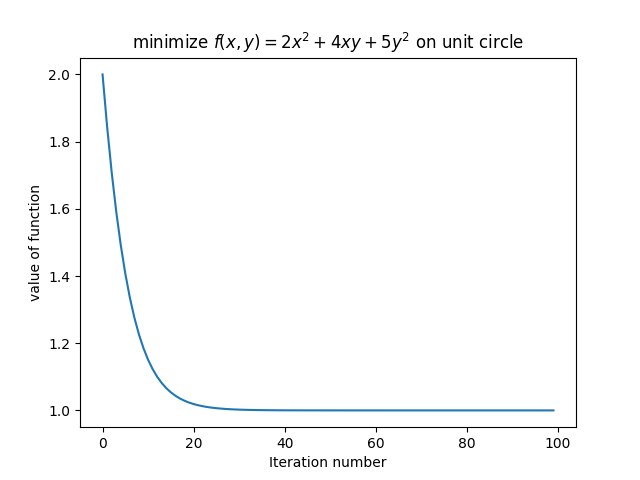
\includegraphics[width = 6.3cm]{Images/result_min.png}
                \end{minipage}
                \begin{minipage}{0.45\hsize}
                    \centering
                    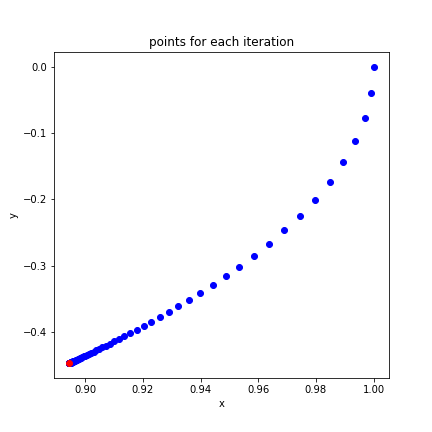
\includegraphics[width = 5.5cm]{Images/eign_vec_min.png}
                \end{minipage}
            \end{tabular}   
        \end{figure}  
    \end{frame}
    \begin{frame}
        \frametitle{実験結果(最大固有値)}
        $q_{A}$の最大値$\lambda_2 = 6$に収束していることが確かめられた.
        また,その時の$x$は$\lambda_2$の固有ベクトル$x_{\lambda_2} = (1/\sqrt{5}, 2/\sqrt{5})$となっている.
        なお, $t = 0.01$, $x_{0} = (1, 0)$とした. 
        \begin{figure}[b]
            \begin{tabular}{c}
                \begin{minipage}{0.55\hsize}
                    \centering
                    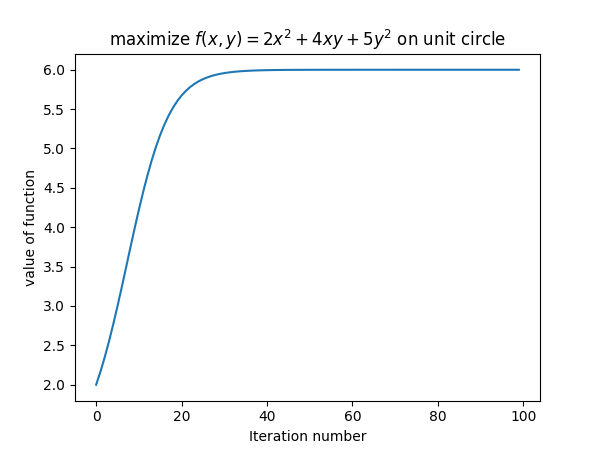
\includegraphics[width = 6.3cm]{Images/result_max.png}
                \end{minipage}
                \begin{minipage}{0.45\hsize}
                    \centering
                    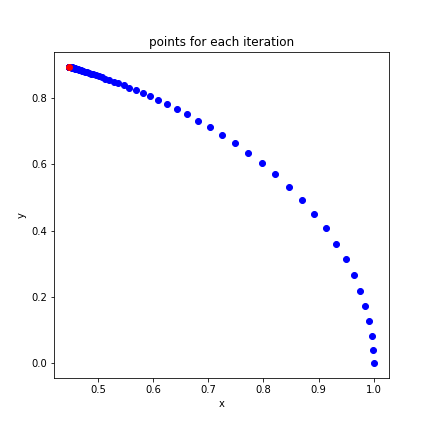
\includegraphics[width = 5.5cm]{Images/eign_vec_max.png}
                \end{minipage}
            \end{tabular}   
        \end{figure}  
    \end{frame}
\section{Optimization Problem on Stiefel Manifold}
    \subsection{Principle Component Analysis}
    \begin{frame}
        \frametitle{データの要約と主成分分析}
        \textbf{主成分分析}(Principle Component Analysis, PCA)とは$n$次元データ$\{x_i\}_{i = 1}^{N}\subset\R^n$をよく表現する正規ベクトル(大きさが1のベクトル)を見つける方法論.
        簡単にいうと, 以下のような赤線を見つけること.
        \begin{figure}
            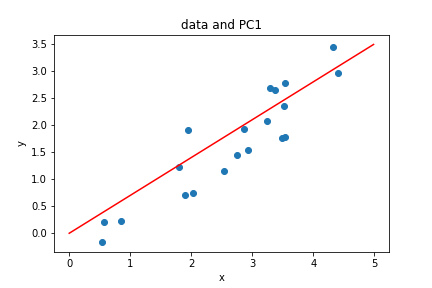
\includegraphics[width=6.0cm]{Images/data_pc1.png}
        \end{figure}
        これ以降, データの平均は0, 分散は1とする. 
    \end{frame}
    \begin{frame}
        \frametitle{赤線の見つけ方}
        正規ベクトル$v_1$が$n$次元データ$\{x_i\}_{i = 1}^{N}\subset\R^n$を一番よく表現(近似)するというのは, 
        $v_1$にデータを射影した時に, 射影前との誤差が最小になるということ. 
        すなわち, $x\in\R^n$の$\operatorname{span}\{v_1\}$への直交射影は
        $v_1v_1^{\top}x$で与えられるから, 
        \begin{align}
            \argmin_{\|v_1\| = 1}\frac{1}{N}\sum_{i = 1}^{N}\|x_i - v_1v_1^{\top}x_i\|^2
        \end{align}
        を求めること!. 
    \end{frame}
    \begin{frame}
        \frametitle{標本共分散行列との繋がり}
        $\|x_i - v_1v_1^{\top}x_i\|^2 = x_i^{\top}x_i - x_i^\top v_1v_1^\top x_i$だから, 先ほどの(1)式は以下と同値.
        \begin{align}
            \argmax_{\|v_1\| = 1}\frac{1}{N}\sum_{i = 1}^{N}x_i^\top v_1v_1^\top x_i
        \end{align}
        ここで, データ$\{x_i\}_{i = 1}^{N}$の平均は0だから, $\{x_i\}_{i = 1}^{N}$の標本共分散行列$C$は
        $C = \frac{1}{N}\sum_{i = 1}^{N}x_ix_i^\top$で与えられるので, 
        \begin{align*}
            \argmax_{\|v_1\| = 1}\frac{1}{N}\sum_{i = 1}^{N}x_i^\top v_1v_1^\top x_i = \argmax_{\|v_1\| = 1}v_1^{\top}Cv_1
        \end{align*}
        となる. $\to$ $C$は対称行列だから, 実はさっきやった問題と同じになる.
    \end{frame}
    \subsection{Stiefel Manifold and PCA}
    \begin{frame}
        \frametitle{第$p$主成分}
        先ほどは, データ$\{x_i\}_{i = 1}^N$を一番近似する正規ベクトル$v_1$を
        求めた. この$v_1$を\textbf{第1主成分}(PC1)という. また, データを2番目によく近似し, $v_1$と直交する
        正規ベクトル$v_2$を\textbf{第2主成分}(PC2)という. 一般に, $v_1, v_2, \ldots, v_{p-1} (p < n)$と直交し,
        データを$p$番目によく近似する正規ベクトル$v_k$を\textbf{第$p$主成分}(PC p)という. 
        \begin{block}{主成分分析} 
            $n$次元データが与えられた時, 上で定めたデータを近似する$1\leq p\leq n$個の
            正規直交基底$\{v_i\}_{i = 1}^p$を求めること.           
        \end{block}
    \end{frame}
    \begin{frame}
        \frametitle{$p$次元への直交射影}
        前スライドより, 主成分$\{v_i\}_{i = 1}^p$を求めるためには以下の最適化問題を解けば良い.
        \begin{align*}
            \argmin_{v_{1}, v_{2}, \ldots, v_{p} : ONS} \frac{1}{N} \sum_{i=1}^{N}\|x_{i}-(v_{1} v_{1}^{T}+\cdots+v_{p} v_{p}^{T}) x_{i}\|^{2}
        \end{align*}
        ここで, $\{v_i\}_{i = 1}^p$は正規直交規定だから$(v_{1} v_{1}^{T}+\cdots+v_{p} v_{p}^{T}) x$は$x\in\R^n$の$\operatorname{span}\{v_1, v_2,\ldots, v_p\}$
        への直交射影である($V = [v_1, v_2, \ldots, v_p]\in\R^{n\times p}$とした時, $V(V^{\top}V)^{-1}V^{\top} = VV^{\top}$). また, $p = 1$の時と同様に考えれば上記の式は
        \begin{align*}
            \argmax_{v_{1}, v_{2}, \ldots, v_{p} : ONS} v_1^{\top}Cv_1 + v_2^{\top}Cv_2 + \cdots + v_p^{\top}Cv_p
        \end{align*}
        と同値. また, ここでトレースの定義より, 以下のようにかける. 
        \begin{align*}
            v_1^{\top}Cv_1 + v_2^{\top}Cv_2 + \cdots + v_p^{\top}Cv_p = \operatorname{tr}(V^{\top}CV)
        \end{align*}  
    \end{frame}
    \begin{frame}
        \frametitle{シュティーフェル多様体と主成分分析}
        前スライドの議論と, シュティーフェル多様体が正規直交基底をなす$n\times p$の集合
        であることを考えれば, 主成分分析は以下のようなシュティーフェル多様体$\operatorname{St}(p, n)$上の
        最適化問題と考えることができる. 
        \begin{exampleblock}{}
            $C$をデータの標本共分散行列とする.
            \begin{mpproblem*}
                \begin{alignat*}{2}
                    &\text{minimize}   & \quad F(X) = - \operatorname{tr}(V^{\top}CV)\\
                    &\text{subject to} & \quad V\in\operatorname{St}(p, n)   
                \end{alignat*}
            \end{mpproblem*}
        \end{exampleblock}   
    \end{frame}
    \subsection{RGD on Stiefel Manifold}
    \begin{frame}
        \frametitle{最適化の準備 : 行列の極分解}
        球面上の二次形式最小化問題の時と同様に, 勾配降下法をシュティーフェル多様体に拡張し
        解くことにする. しかし, これまた球面上に拡張した時と同様に$x - t\mathrm{grad}F(X)\notin\operatorname{St}(p, n)$と
        なる問題が発生する. 今回は, これを解決するために行列の極分解(polar decomposition)を利用する.
        \begin{prop}[行列の極分解]
            任意の実行列$A\in\R^{m\times n}$は直交行列$U$と半正定値対称行列$P$を用いて
            \begin{align*}
                A = UP
            \end{align*}
            と分解できる. 
        \end{prop}
    \end{frame}
    \begin{frame}
        \frametitle{シュティーフェル多様体上の勾配降下法}
        \begin{algorithm}[H]
            \caption{Riemannian Gradient Decent on Stiefel Manifold}
            \begin{algorithmic}
                \REQUIRE $F$: differentiable function on $\operatorname{St}(p, n)$
                \REQUIRE $0< t <1$ : 
                \STATE $X\leftarrow X_{0}\in\operatorname{St}(p, n)$
                \WHILE{$X$ not converged} 
                \STATE $d = -t~\mathrm{grad} F(X)$
                \STATE $X\leftarrow (X + d)(\mathbb{I}_{p} + d^{\top}d)^{-1/2}$ 
                \ENDWHILE
                \RETURN $X$
            \end{algorithmic}
        \end{algorithm}
        なお, アルゴリズム中の$(X + d)(\mathbb{I}_{p} + d^{\top}d)^{-1/2}$が, $X + d$の
        極分解の$U$に対応している. 
    \end{frame}
    \begin{frame}
        \frametitle{シュティーフェル多様体上の勾配の求め方}
        \begin{prop}[シュティーフェル多様体の勾配と直交射影]
            目的関数$F:\R^{n\times p}\to\R$を$\operatorname{St}(p, n)$に制限した関数を$\overline{F}:\operatorname{St}(p, n)\to\R$
            とする. この時, $X\in\operatorname{St}(p, n)$について, $P_X : T_{X}\R^{n\times p}\to T_{x}\operatorname{St}(p, n)$を
            $T_{X}\R^{n\times p} = \R^{n\times p}$から閉部分空間$T_{X}\operatorname{St}(p, n)$への直交射影とすれば,
            \begin{align*}
                \mathrm{grad} \overline{F}(x) = P_{X}(\mathrm{grad}_{\R^{n\times p}}F(X))
            \end{align*}
            が成立する. また, 直交射影$P_X$は 
            \begin{align*}
                P_{X}(\xi)=\left(I-X X^{T}\right) \xi+X \operatorname{skew}\left(X^{T} \xi\right)
            \end{align*}
            で与えられる. ただし, $\operatorname{skew}(A) = \frac{1}{2}(A - A^\top)$.
        \end{prop}
    \end{frame}
    \section*{Conclution}
    \begin{frame}
        \frametitle{興味が出てきた人のために}
        \begin{enumerate}
            \item 球やシュティーフェルの他にも, 実問題では Grassmann Manifoldなど他の多様体も登場する.
            \item アルゴリズムに出てきた, 集合に戻すという写像をレトラクション(Retraction)という形で一般化される\cite{absil}. 
            \item 最近, 一部のリーマン多様体においてレトラクションがいらないという話が出てきた\cite{noretract}.
        \end{enumerate}
    \end{frame}
\section*{References}
    \begin{frame}\frametitle{References}
        \begin{thebibliography}{9}
            \beamertemplatetextbibitems
            \bibitem{absil} P.-A. ABSIL, R. MAHONY, AND R. SEPULCHRE, Optimization Algorithms on Matrix Manifolds, 
                       Princeton University Press, Princeton, NJ, 2008.
            \bibitem{qform} https://www.cck.dendai.ac.jp/math/support/advance/2次形式.pdf, 東京電機大学
            \bibitem{sato} 佐藤 寛之, 曲がった空間での最適化, 日本オペレーションズ・リサーチ学会, オペレーションズ・リサーチ Vol.60 9月号, 2015
            \bibitem{satoi} 佐藤一宏, 線形数理要論(第8回), \url{http://www.kazuhirosato.work/entry/senkeisuriyoron_2020}, 2020
            \bibitem{noretract} Pierre Ablin and Gabriel Peyré, Fast and accurate optimization on the orthogonal manifold without retraction, \url{https://arxiv.org/abs/2102.07432}, 2021
	    \end{thebibliography}
    \end{frame}
\end{document}


